\documentclass[journal,12pt,twocolumn]{IEEEtran}

\usepackage{setspace}
\usepackage{gensymb}


\singlespacing

\usepackage[cmex10]{amsmath}
%\usepackage{amsthm}
%\interdisplaylinepenalty=2500
%\savesymbol{iint}
%\usepackage{txfonts}
%\restoresymbol{TXF}{iint}
%\usepackage{wasysym}
\usepackage{amsthm}

\usepackage{mathrsfs}
\usepackage{txfonts}
\usepackage{stfloats}
\usepackage{bm}
\usepackage{cite}
\usepackage{cases}
\usepackage{subfig}

\usepackage{longtable}
\usepackage{multirow}

\usepackage{enumitem}
\usepackage{mathtools}
\usepackage{steinmetz}
\usepackage{tikz}
\usepackage{circuitikz}
\usepackage{verbatim}
\usepackage{tfrupee}
\usepackage[breaklinks=true]{hyperref}

\usepackage{tkz-euclide} %loads TikZ and tkz-base

\usetikzlibrary{calc,math}
\usepackage{listings}
    \usepackage{color}                                          
    \usepackage{array}                                          
    \usepackage{longtable}                                      
    \usepackage{calc}                                          
    \usepackage{multirow}                                      
    \usepackage{hhline}                                        
    \usepackage{ifthen}
    \usepackage{lscape}    
\usepackage{multicol}
\usepackage{chngcntr}

\DeclareMathOperator*{\Res}{Res}

\renewcommand\thesection{\arabic{section}}
\renewcommand\thesubsection{\thesection.\arabic{subsection}}
\renewcommand\thesubsubsection{\thesubsection.\arabic{subsubsection}}

\renewcommand\thesectiondis{\arabic{section}}
\renewcommand\thesubsectiondis{\thesectiondis.\arabic{subsection}}
\renewcommand\thesubsubsectiondis{\thesubsectiondis.\arabic{subsubsection}}

\hyphenation{op-tical net-works semi-conduc-tor}
\def\inputGnumericTable{}                                 %%

\lstset{
%language=C,
frame=single,
breaklines=true,
columns=fullflexible
}

\begin{document}

\newtheorem{theorem}{Theorem}[section]
\newtheorem{problem}{Problem}
\newtheorem{proposition}{Proposition}[section]
\newtheorem{lemma}{Lemma}[section]
\newtheorem{corollary}[theorem]{Corollary}
\newtheorem{example}{Example}[section]
\newtheorem{definition}[problem]{Definition}

\newcommand{\BEQA}{\begin{eqnarray}}
\newcommand{\EEQA}{\end{eqnarray}}
\newcommand{\define}{\stackrel{\triangle}{=}}
\bibliographystyle{IEEEtran}
\providecommand{\mbf}{\mathbf}
\providecommand{\pr}[1]{\ensuremath{\Pr\left(#1\right)}}
\providecommand{\qfunc}[1]{\ensuremath{Q\left(#1\right)}}
\providecommand{\sbrak}[1]{\ensuremath{{}\left[#1\right]}}
\providecommand{\lsbrak}[1]{\ensuremath{{}\left[#1\right.}}
\providecommand{\rsbrak}[1]{\ensuremath{{}\left.#1\right]}}
\providecommand{\brak}[1]{\ensuremath{\left(#1\right)}}
\providecommand{\lbrak}[1]{\ensuremath{\left(#1\right.}}
\providecommand{\rbrak}[1]{\ensuremath{\left.#1\right)}}
\providecommand{\cbrak}[1]{\ensuremath{\left\{#1\right\}}}
\providecommand{\lcbrak}[1]{\ensuremath{\left\{#1\right.}}
\providecommand{\rcbrak}[1]{\ensuremath{\left.#1\right\}}}
\theoremstyle{remark}
\newtheorem{rem}{Remark}
\newcommand{\sgn}{\mathop{\mathrm{sgn}}}
\providecommand{\abs}[1]{\left\vert#1\right\vert}
\providecommand{\res}[1]{\Res\displaylimits_{#1}}
\providecommand{\norm}[1]{\left\lVert#1\right\rVert}
%\providecommand{\norm}[1]{\lVert#1\rVert}
\providecommand{\mtx}[1]{\mathbf{#1}}
\providecommand{\mean}[1]{E\left[ #1 \right]}
\providecommand{\fourier}{\overset{\mathcal{F}}{ \rightleftharpoons}}
%\providecommand{\hilbert}{\overset{\mathcal{H}}{ \rightleftharpoons}}
\providecommand{\system}{\overset{\mathcal{H}}{ \longleftrightarrow}}
%\newcommand{\solution}[2]{\textbf{Solution:}{#1}}
\newcommand{\solution}{\noindent \textbf{Solution: }}
\newcommand{\cosec}{\,\text{cosec}\,}
\providecommand{\dec}[2]{\ensuremath{\overset{#1}{\underset{#2}{\gtrless}}}}
\newcommand{\myvec}[1]{\ensuremath{\begin{pmatrix}#1\end{pmatrix}}}
\newcommand{\mydet}[1]{\ensuremath{\begin{vmatrix}#1\end{vmatrix}}}
\numberwithin{equation}{subsection}
\makeatletter
\@addtoreset{figure}{problem}
\makeatother
\let\StandardTheFigure\thefigure
\let\vec\mathbf
\renewcommand{\thefigure}{\theproblem}
\def\putbox#1#2#3{\makebox[0in][l]{\makebox[#1][l]{}\raisebox{\baselineskip}[0in][0in]{\raisebox{#2}[0in][0in]{#3}}}}
     \def\rightbox#1{\makebox[0in][r]{#1}}
     \def\centbox#1{\makebox[0in]{#1}}
     \def\topbox#1{\raisebox{-\baselineskip}[0in][0in]{#1}}
     \def\midbox#1{\raisebox{-0.5\baselineskip}[0in][0in]{#1}}
\vspace{3cm}
\title{Assignment 5}
\author{Priya Bhatia}
\maketitle
\newpage
%\tableofcontents
\bigskip
\renewcommand{\thefigure}{\theenumi}
\renewcommand{\thetable}{\theenumi}
\begin{abstract}
This document finds the normal at the given point on the curve
\end{abstract}
%
Download python codes from 
%
\begin{lstlisting}
https://github.com/priya6971/matrix_theory_EE5609/tree/master/Assignment5/codes
\end{lstlisting}
%
%
Download latex-tikz codes from 
%
\begin{lstlisting}
https://github.com/priya6971/matrix_theory_EE5609/tree/master/Assignment5
\end{lstlisting}
%
\section{\textbf{Problem}}
Find the normal at the point $\myvec{1\\1}$ on the curve $2y + x^2 = 3$
\section{\textbf{Solution}}
Given, 
\begin{align}
	x^2 + 2y - 3 &= 0 \label{eq:eq1}
\end{align}
From \eqref{eq:eq1}, 
\begin{align} 
    \vec{V} &= \myvec{1 & 0 \\ 0 & 0} \label{eq:eq2} \\
    \vec{u} &= \myvec{0 \\ 1} \\
    f &= -3
\end{align}
From \eqref{eq:eq2},
\begin{align}
    \mydet{V} = \mydet{1 & 0 \\ 0 & 0} = 0 \label{eq:eq3}
\end{align}
Now \eqref{eq:eq3} implies that the curve is a parabola. We can find the Eigen values corresponding to the $\vec{V}$,
\begin{align}
    \mydet{V-\lambda I} &= 0 \nonumber \\
    \mydet{1-\lambda & 0 \\ 0 & -\lambda} &= 0 \nonumber \\
    \implies \lambda &= 0,1 \label{eq:eq4}
\end{align}
Calculating the Eigen Vectors corresponding to $\lambda=0,1$ respectively,
\begin{align}
    \vec{V}\vec{x} = \lambda\vec{x} \nonumber 
\end{align}
\begin{align}
    \myvec{1 & 0 \\ 0 & 0}\vec{x} = 0;\implies \vec{p}_1 = \myvec{0 \\ 1} \label{eq:eq5} \\
    \myvec{0 & 0 \\ 0 & -1}\vec{x} = 0;\implies \vec{p}_2 = \myvec{1 \\ 0} \label{eq:eq6}
\end{align}
By Eigen decomposition on $\vec{V}$,
\begin{align}
    \vec{V} = \vec{P}\vec{D}\vec{P}^T \nonumber \\
    where, \vec{P} = \myvec{\vec{p}_1 & \vec{p}_2} = \myvec{0 & 1 \\ 1 & 0} \label{eq:eq7} \\
    \vec{D} = \myvec{\lambda_1 & 0 \\ 0 & \lambda_2} = \myvec{0 & 0 \\ 0 & 1} \label{eq:eq8}
\end{align}
To find the vertex of the parabola,
\begin{align}
    \myvec{\vec{u}^T+\eta \vec{p}_1^T \\ \vec{V}}\vec{c} = \myvec{-f \\ \eta \vec{p}_1-\vec{u}} \label{eq:eq9} \\
    where, \eta = \vec{u}^T\vec{p}_1 = 1 \label{eq:eq10}
\end{align}
Substituting values from \eqref{eq:eq2}, \eqref{eq:eq5} and \eqref{eq:eq10} in \eqref{eq:eq9}, 
\begin{align}
    \myvec{0 & 2 \\ 1 & 0 \\ 0 & 0}\vec{c}=\myvec{3 \\ 0 \\ 0} \label{eq:eq11}
\end{align}
Removing last row and representing \eqref{eq:eq11} as augmented matrix and then converting the matrix to echelon form,
\begin{align}
    \myvec{0 & 2 & 3 \\ 1 & 0 & 0} \xleftrightarrow[]{R_1\leftrightarrow R_2} \myvec{1 & 0 & 0 \\ 0 & -2 & -3}\\
    \myvec{1 & 0 & 0 \\ 0 & -2 & -3} \xleftrightarrow[]{R_2\leftarrow -\frac{R_2}{2}} \myvec{1 & 0 & 0 \\ 0 & 1 & \frac{3}{2}}\label{eq:eq12}
\end{align}
From \eqref{eq:eq12} it can be observed that,
\begin{align}
    \vec{c} = \myvec{0 \\ \frac{3}{2}} \label{eq:eq13}
\end{align}
Now to evaluate the direction vector $\vec{m}$,
\begin{align}
    \vec{m}^T(\vec{V}\vec{q} + \vec{u}) &= 0 \\
    \vec{m}^T\myvec{\myvec{1 & 0 \\ 0 & 0}\myvec{1 \\ 1} +\myvec{0 \\ 1}} &= 0 \\
    \vec{m}^T\myvec{\myvec{1 \\ 0} +\myvec{0 \\ 1}} &= 0 \\
    \vec{m}^T\myvec{1 \\ 1} &= 0 \\
    \implies \vec{m} &= \myvec{1 \\ -1} \label{eq:eq14}
\end{align}
Now to obtain the equation of normal using,
\begin{align}
    \vec{m}^T(\vec{x} - \vec{q}) &= 0 \\
    \myvec{1 & -1}\myvec{\vec{x} - \myvec{1 \\ 1}} &= 0 \\
    \myvec{1 & -1}\vec{x} &= 0 
\end{align}
\begin{figure}[h!]
\centering
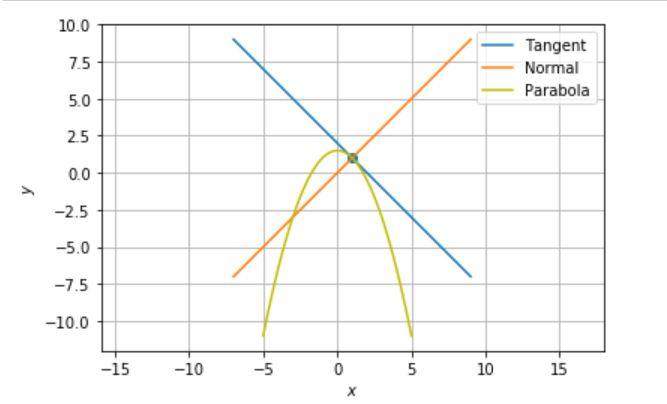
\includegraphics[width=\columnwidth]{Plot.JPG}
\caption{{Parabola showing tangent perpendicular to the normal}}
\label{myfig}
\end{figure}
\end{document}